%!TeX root = 6-perspectives.tex
\documentclass[main]{subfiles}

\begin{document}

\chapter{Toward the next generation of screenings}
\vspace*{-1\baselineskip}

\section{Limits of the Current Screening Methodologies}

As presented in our review of the different screening methodologies in the chapter 1, it is very common to screen for one particular metric whether it is the selectivity or the permselectivity or the capacity depending on the targeted application. Attempts of screening that searches for the most selective materials but combined with a good capacity are more and more common.\autocite{Chung_2019,Zhang_2022,Solanki_2020} If we take the problem of the selectivity screening, many improvements can be made in terms of calculation efficiency, or in terms of correctness of the molecular description. In the previous chapters, I mostly focused on the gain in efficiency by exploring many adsorption energy sampling techniques and by comparing their computational time as well as their accuracy. But I also started to incorporate other properties to the screening procedure by exploring the transport properties for instance. And in an effort to always aim at better efficiency, I explored alternative calculation strategies in addition to the more standard ones. 

To further improve the shortcomings of the current adsorption screening methodologies, we need to explore even more material properties. For example, the rigidity of the structures in most of the screening procedures could sometimes mislead toward materials that appear to have a very high selectivity, whereas the flexible nature of the material tend to lower the calculated selectivity. By taking into account flexibility, one could completely change the rankings found by the screening and hence finding other maybe better materials through this new approach. The other property that could completely change the results obtained by current methodologies is the polarization. For adsorbates like xenon and krypton, the difference in polarizability is in fact at the origin of the separability of these gas using an adsorbent material. A better description of this particular property can in fact completely change the results of the screening. If we look at the best experimental materials, they are either decorated with polar groups like in the article~\cite{Li_2019} or they present open metal sites like in the article~\cite{Pei_2022}. However, we do not find these criteria as being essential when looking at the results of the current screenings. 

In this final chapter, I want to discuss three main research focuses: (i) the calculation of transport properties that could be further optimized, (ii) the adsorption calculations in flexible frameworks, and (iii) the better description of the polarization in the energy calculations.

\section{Future Developments on Transport Properties}

\subsection{Finish the optimized version of TuTraST}

Next steps in the development of the C++ tool

Layer-by-layer growth 
equivalent to find the equidistant points within $E$ and $E+\delta E$. 
Lionel Zoubritzky

\subsection{Connection to the breakthrough experiments}

\begin{figure}[ht]
  \centering
  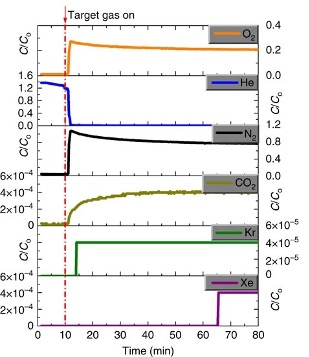
\includegraphics[width=0.4\textwidth]{figures/6-perspectives/sbmof_breakthrough.jpg}
  \caption{ Experimental breakthrough curves in SBMOF-1 for a gas mixture with 400 ppm Xe and 40 ppm Kr balanced with dry air. Reprinted with permission from Ref.~\cite{Banerjee_2016} copyright \copyright\ 2016 Springer Nature. }\label{fgr:sbmof_breakthrough}
\end{figure}

Diffusion coefficients 

RUPTURA, breakthrough curve
\todo{one test with SBMOF-1 (experimental?)}
Discuss the different parameters, and their relevance.

PSA for separation most commonly used: selectivity, working capacity, regenerability (kinetics and energy used to regenerate the material i.e., empty the pores for another cycle).\autocite{Kumar_1994}

\section{Screening flexible materials}

The reason why people usually prefer rigid frameworks is the high complexity brought by the simulation of the dynamics of a flexible framework. We already saw the cost of simulating a grand canonical ensemble using MC methods and developed strategies to avoid these types of calculations. The simulation of a flexible framework would require to relax the volume and simulate an osmotic ensemble ($\mu$,$P$,$T$), which requires MC moves on the volume of the unit cell itself.\autocite{Bousquet2012} This type of MC simulation describes more accurately every aspect of the flexibility be it the intrinsic flexibility due to thermal agitation or the adsorbate-induced flexibility. However, in a screening procedure, this type of simulation can be prohibitively long, it should, however, be used as an accurate method to confirm the properties of a few top materials. 

In order to incorporate flexibility effects in the screening procedure at a minimal computational cost, another approach is to use a set of rigid structures that reflects the structural diversity generated by the thermal agitation of the nanoporous material. A first study on the effect of this intrinsic flexibility on the Xe/Kr selectivity suggests that some materials could lose selectivity due to the less favorable pore size the structure vibrates.\autocite{Witman_2017} For instance, the authors explained the discrepancies between the experimental and theoretical Xe/Kr selectivity of KAXQIL\autocite{KAXQIL} by its intrinsic flexibility, which questions the performance ranking obtained by a rigid-framework screening. In this section, I will introduce in detail the study of Witman et al.\autocite{Witman_2017} and I will especially focus on the case of KAXQIL presented by them. Then, I will present introduce another approach based on the structural diversity among similar deposited experimental structures. We can in fact count a dozen different structures with the same chemical nature as KAXQIL but with very different structural characteristics depending on the loaded adsorbate, which suggests an adsorbate-induced flexibility in addition to the intrinsic flexibility previously studied. 

\subsection{Snapshot method}

\subsubsection{Methodology}

To model the dynamics of the framework, Witman et al.\ use the UFF forcefield to describe the non-electrostatic framework bond potentials except for the metal bonding. For the bond dynamics around the metal, a harmonic equilibrium is fixed around the values extracted from the experimental structure. For this reason, this forcefield definition is referred to as the UFF-fix-metal (UFF-FM). In addition of the Lennard-Jones description, the point charge Coulomb interactions are described using the standard Ewald summation technique based on the charges calculated by the density derived electrostatic and chemical (DDEC) method.\autocite{manz2010chemically} Using this forcefield, the authors carried out a systematic snapshot generation of the structures from the CoRE MOF 2014 database with pre-calculated DDEC charges. And these snapshots were used to determine flexible Xe and Kr Henry constant values as well as the infinite dilution Xe/Kr selectivity. The flexible selectivity was found to be lower for {95\%} of the materials with a rigid selectivity over $25$ (as shown on the Figure~\ref{fgr:underestimated_rigid}), which suggests an overestimation of the top performing materials. Furthermore, the effect of flexibility is much more important for the smaller pore sizes, because of the intensity of the interactions at lower distance. 

\begin{figure}[ht]
  \centering
  \begin{subfigure}[b]{0.32\textwidth}
    \centering
    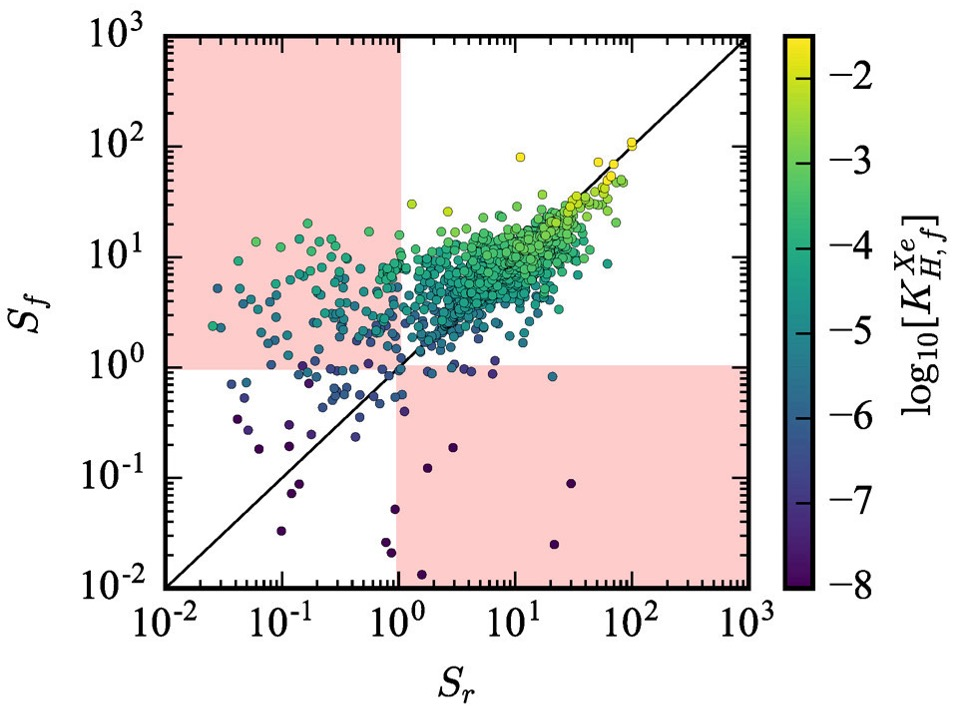
\includegraphics[width=\textwidth]{figures/6-perspectives/s_f-s_r.jpg}
    \caption{Flexible \emph{vs.} Rigid}
  \end{subfigure}
  \hfill
  \begin{subfigure}[b]{0.3\textwidth}
    \centering
    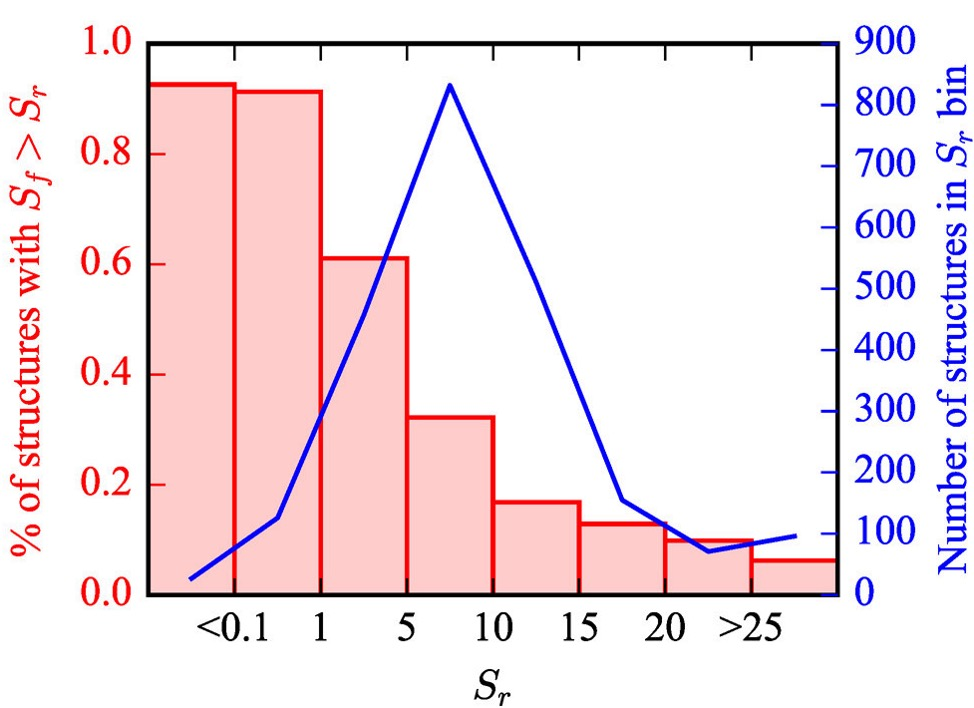
\includegraphics[width=\textwidth]{figures/6-perspectives/histogram_flex.jpg}
    \caption{selectivity underestimation}\label{fgr:underestimated_rigid}
  \end{subfigure}
  \hfill
  \begin{subfigure}[b]{0.32\textwidth}
    \centering
    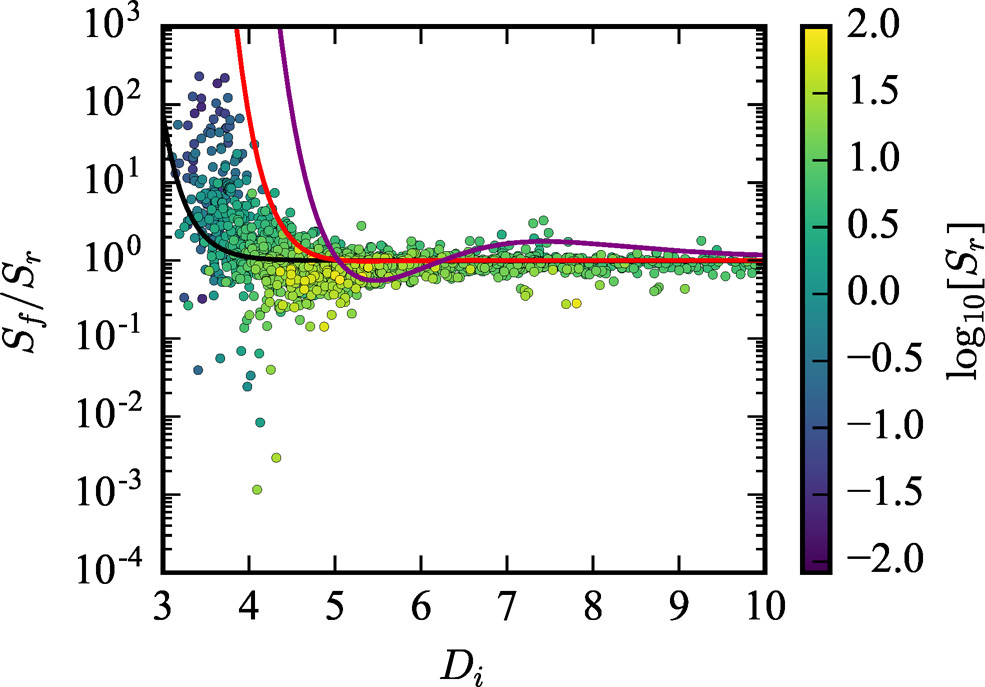
\includegraphics[width=\textwidth]{figures/6-perspectives/s_ratio_LCD.jpg}
    \caption{Flexibility effect \emph{vs.} LCD}
  \end{subfigure}
  \caption{ (a) A scatter plot of the flexible selectivity against the rigid selectivity labeled by the log$_10$ of the flexible Xe Henry constants. (b) Barplot of the fraction of the underestimated selectivity ($s_f>s_r$) for different categories of materials going from the least selective ones to the most selective ones ($s_r>25$). (c) Effect of the flexibility measured using the ratio $s_f/s_r$ as a function of the largest included sphere diameter. The line plots correspond to analytical modeling of the effect that will not be detailed here. Reprinted with permission from the original paper~\cite{Witman_2017} copyright \copyright\ 2017 American Chemical Society. }\label{fgr:flexibility_study}
\end{figure}

If we now focus on the issue of flexibility in KAXQIL, the authors used several methods to evaluate its effect on the Xe and Kr Henry constants and the Xe/Kr selectivity. For instance, they used another description of the metal--ligand bond using a cationic dummy model (UFF-CDM) and an \emph{ab initio} MD simulation using the PBE DFT function,\autocite{Perdew_1996} with a Grimme's D3 van der Waals correction\autocite{Grimme_2010} (PBE+D3). Each of these three methods are used to generate about $30$ snapshots that were eventually used to determine the flexible framework's adsorption properties for KAXQIL.

The authors found that the lower experimental selectivity value of $16$ compared to the UFF-determined one could be partially explained by a flexibility effect. The selectivity evaluated on a rigid SBMOF-1 structure using the standard UFF forcefield is way higher than the one obtained when considering snapshots of a vibrating structure. The \emph{ab initio} MD method that should be the closest to the actual dynamics does not recover the whole phenomenon because of the system size dependence. To actually see the crystallographic deformations, multiple unit cell replications are usually necessary. Moreover, the UFF forcefield used does not give a perfect picture of the interaction energies at play in the system neither. But an overall trend is, however, drawn in this study since it is possible to attribute the discrepancies between experimental and theoretical data to the rigidity hypothesis.

\begin{table}[t]
  \centering
  \small
  \begin{tabular}{|l|c|c|c|c|}
  \hline
    Data source & Flexible &  Xe Henry Constant &  Kr Henry Constant &  Xe/Kr \\
      & structure &  \si{\mmol\per\g\per\Pa} &  \si{\mmol\per\g\per\Pa} &  selectivity \\
  \hline
    Experimental data\autocite{Banerjee_2016} & maybe &  $3.84\times 10^{-4}$ &  $2.37\times 10^{-5}$ &  $16$ \\
  \hline
    Rigid structure SBMOF-1\autocite{Banerjee_2016} & no &  $1.45\times 10^{-2}$ &  $2.70\times 10^{-4}$ &  $54$ \\
    PBE+D3 (2,2,1 unit cell) & yes &  $6.80\times 10^{-3}$ &  $1.77\times 10^{-4}$ &  $38$ \\
    UFF-FM & yes &  $6.24\times 10^{-3}$ &  $1.67\times 10^{-4}$ &  $37$ \\
    UFF-DCM & yes &  $3.18\times 10^{-3}$ &  $1.28\times 10^{-4}$ &  $25$ \\
  \hline
\end{tabular}
\caption{ Results of the flexibility analysis carried out by Witman et al., flexibility reduces the values originally calculated in a rigid structure. Reproduced with permission from the original paper~\cite{Witman_2017} copyright \copyright\ 2017 American Chemical Society.}
\label{table:witman_sbmof}
\end{table}

This approach does not give a complete picture of the flexibility effect on the selectivity value, but can rapidly identify a weakness in the rigidity hypothesis and therefore warn on a possible over- or under-estimation of the selectivity, which can lead to identifying wrongfully a material as the best or missing the opportunity of finding a better material. The main advantage of this technique is the relative speed compared to an osmotic ensemble Monte Carlo simulation.\autocite{Bousquet2012} But the main drawback is the imperfect description of the intrinsic flexibility as the only phenomenon at play. For instance, in the following, I will show some adsorbate-induced effects that were neglected but can be retrieved by using the multiple works on the same SBMOF-1 material. In this approach, we avoid the issues around MD simulations and we only base our reasoning on observed structural changes. 


\subsection{Experimental database approach}

According to original paper on SBMOF-1,\autocite{Banerjee_2016} the theoretical selectivity calculated by UFF is around $70.6$. However, the experimental selectivity is much lower, around $16$. To solve this mystery, Witman et al. used a snapshot-based method to evaluate the effect of selectivity. The intrinsic flexibility lowers the selectivity, which goes in the right direction to explain the difference of selectivity, but it does not seem to capture the whole picture. 

I think that the missing effect that could explain the discrepancies observed is the deformation induced by the loading of adsorbate inside the material. For instance, experimentally a structure is never empty when we resolve it by X-ray, and molecules are actually loaded inside. As shown on the Table~\ref{table:sbmof}, the structure that was originally published for its good \ce{CO2}/\ce{N2} selectivity\autocite{Yeh2012,Banerjee2012} was also tested for water adsorption, and two different structures emerged from this study: KAXQOR and KAXQIL. The first one is loaded by either air or \ce{CO2}, and the structure does not seem to be stretched as much (low LCD values around \SI{4.5}{\angstrom}). The second one, on the other hand, is loaded by water that forms big clusters inside the pores and therefore stretches the pore size toward higher values (high LCD values around \SI{5.0}{\angstrom}). If we look at the structures resolved in the Nature Communications study\autocite{Banerjee_2016}, depending on the adsorbate (hexane, water, butane, krypton or xenon), the LCD and PLD values change in the first order according to the size of the adsorbate as illustrated on the Figure~\ref{fgr:stretch}. There are, of course, other effects, like the clustering we mentioned for water, but also less expected effects such as the orientation of the adsorbate inside the structure. 

\begin{table}[t]
\centering
\setlength\extrarowheight{2pt}
\small
\begin{tabular}{|l|r|c|c|c|c|}
  \hline
  Experimental structure & Adsorbate in &  Selectivity &  LCD (\SI{}{\angstrom}) &  PLD (\SI{}{\angstrom}) &  Xe Diff. \\
  CCSD ref. code & the structure &  $s\ex{Xe/Kr}_0$ &   &   & Coeff. \si{\square\cm\per\s} \\
  \hline
  KAXQOR01\autocite{Yeh2012} & Not specified & 101 & 4.99 & 3.66 & 3$\times$10\ex{-09} \\
  KAXQOR\autocite{Banerjee2012} & Not specified & 22 & 4.51 & 4.04 & 7$\times$10\ex{-06}  \\
  KAXQIL\autocite{Banerjee2012} & H$_2$O & 104 & 5.12 & 3.77 & 3$\times$10\ex{-08} \\
  QUXRIM\autocite{Banerjee2016hydro} & hexane &  52 & 4.75 & 4.31 & 3$\times$10\ex{-05}  \\
  QUXRUY\autocite{Banerjee2016hydro} & hexane &  96 & 4.91 & 3.57 & 9$\times$10\ex{-10} \\
  QUXROS\autocite{Banerjee2016hydro} & hexane &  99 & 5.00 & 3.66 & 5$\times$10\ex{-09}  \\
  QUXREI\autocite{Banerjee2016hydro} & hexane & 101 & 5.02 & 3.67 & 7$\times$10\ex{-09}  \\
  QUXRAE\autocite{Banerjee2016hydro} & hexane & 100 & 5.03 & 3.68 & 7$\times$10\ex{-09}  \\
  QUXQUX\autocite{Banerjee2016hydro} & butane & 103 & 5.17 & 3.83 & 1$\times$10\ex{-07}   \\
  QUWYEO\autocite{Banerjee2016hydro} & butane & 100 & 4.99 & 3.65 & 5$\times$10\ex{-09} \\
  \hline  
  UQEFAZ\autocite{Banerjee_2016} & krypton & 23 & 4.53 & 4.08 & 5$\times$10\ex{-06}   \\
  UQEFED\autocite{Banerjee_2016} & xenon & 63 & 4.89 & 3.54 & 1$\times$10\ex{-11}   \\
  \hline
  \end{tabular}
  \caption{ \todo{add Henry} Structural, adsorption and transport properties of structures in the CSD database that are similar to SBMOF-1\autocite{Banerjee_2016}. The last structures actually correspond to the structures resolved in the paper presenting SBMOF-1 in Nature Communications. We can note the structural diversity that induces this diversity of properties. (The pore sizes are calculated using the CCDC radii definition.) }
  \label{table:sbmof}
\end{table}

As shown on the Figure~\ref{fgr:ads_config}, the orientation of the hexane molecule inside the material seems to favor either a configuration with a large LCD and a low PLD (QUXRUY), or a slightly lower LCD with a slightly higher PLD (QUXRIM). The material configurations are, however, a bit different from the ones observed with KXQOR or KAXQIL. 

\begin{figure}[ht]
  \centering
  \begin{subfigure}[b]{0.45\textwidth}
    \centering
    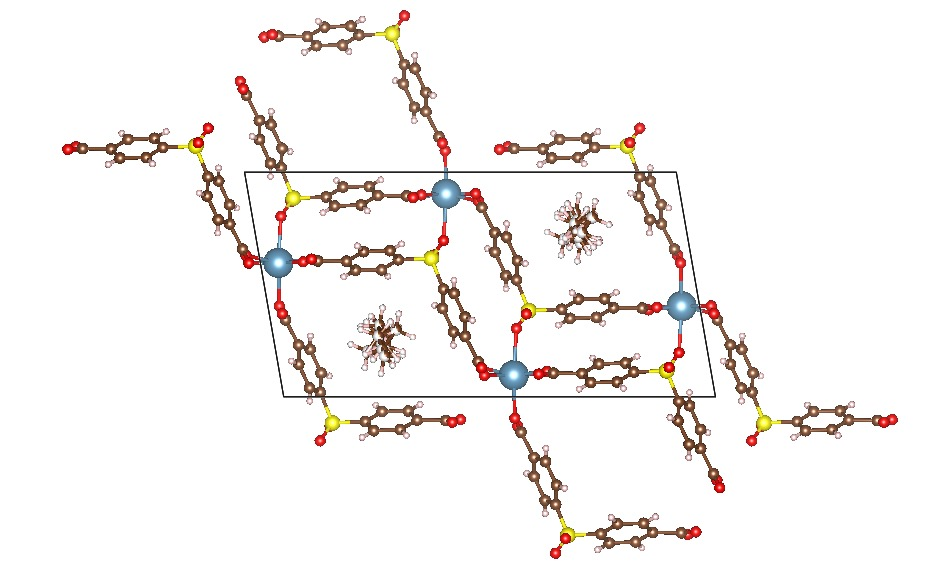
\includegraphics[height=0.6\textwidth]{figures/6-perspectives/QUXRIM.jpg}
    \caption{QUXRIM}\label{fgr:QUXRIM}
  \end{subfigure}
  \hfill
  \begin{subfigure}[b]{0.45\textwidth}
    \centering
    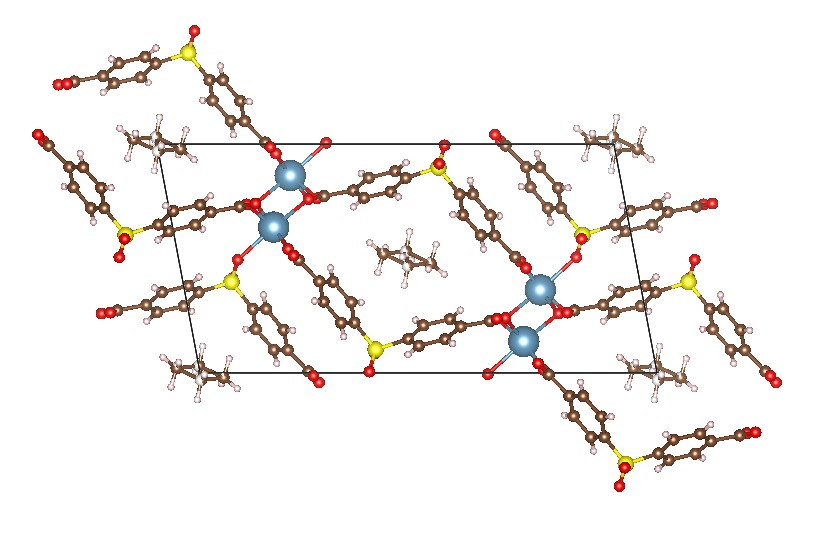
\includegraphics[height=0.6\textwidth]{figures/6-perspectives/QUXRUY.jpg}
    \caption{QUXRUY}\label{fgr:QUXRUY}
  \end{subfigure}
  \caption{ An illustration of the effect of the orientation of hexane inside a SBMOF-1-like material. In QUXRIM (a), the carbon atoms are oriented toward the S atoms, whereas in QUXRUY (b) they are oriented toward the Ca atoms. This difference in the orientation could explain the different structural properties of the materials reported on the Table~\ref{table:sbmof}. Color code: brown for C, white for H, red for O, cyan for Ca, yellow for S. The structure visualizations are generated using the VESTA software.\autocite{VESTA}}\label{fgr:ads_config}
\end{figure}

Now that I characterized the adsorbate effect on a few example configurations, we can better understand the thought process that leads to the identification of KAXQIL as a candidate for Xe/Kr separation. The KAXQIL structure is actually representing the material loaded by water with large pores which enables a good interaction with a large molecule like xenon. For this reason, it was identified as a top selective material. However, when it was experimentally tested for low-pressure adsorption using the Henry constant, it is most likely that the pores are not stretched, which implies lower Henry constants than expected. The structures UQEFAZ or KAXQOR seem to a better description of this low-pressure case since the experimental selectivity values are much more consistent with their theoretical selectivity values. 

To confirm this hypothesis, we would need to measure a high-loading Xe/Kr binary mixture adsorption uptake. If xenon is highly represented in the adsorbent material, then the structure would be much more favorable to the xenon adsorption, hence increasing the selectivity value closer to the theoretically predicted one. This also highlights a composition effect, if the initial mixture has a low xenon content, the structure would most likely have narrower pores, which could decrease the selectivity. By changing the composition of the binary mixture, this effect could also be measured experimentally if the initial hypothesis on the adsorbate-induced flexibility is correct.

This method could be used on other materials by screening for materials with a similar chemical composition and topology, for example. However, due to the bias in research focus, it is not always possible to find structures in very different adsorption conditions. To work around these limitations, one could either experimentally generate these structures when a material seems interesting to see if the flexibility plays a role in the adsorption process. Alternatively, one could computationally generate these structures by running structure optimizations on loaded structures. Either way, this new approach to flexibility seems complementary to the ones mentioned previously because it seems to have a similar (or slightly higher due to the adsorbate) computational cost as the Witman approach, while avoiding the computationally prohibitive calculation (in a screening) presented by Bousquet et al. 


\subsubsection{Diffusion in a flexible environment}

The transport can also be modulated by the adsorbate-induced flexibility of SBMOF-1. Depending on the structural configuration of the material, the diffusion coefficient is limiting only for some configurations of the material: it is equal to $3\times10^{-8}$~\si{\square\cm\per\s} for KAXQIL and $1\times10^{-11}$~\si{\square\cm\per\s} for UQEFED (Table~\ref{table:sbmof}). This lower diffusion coefficient can be simply explained by the change in PLD value induced by the stretching illustrated on the Figure~\ref{fgr:stretch}. For a material mostly loaded by krypton molecules, the diffusion coefficient of xenon is much higher ($5\times10^{-6}$~\si{\square\cm\per\s}), although it not free diffusion, it can at least be considered as an unobstructed diffusion inside the material. 

\begin{figure}[ht]
  \centering
  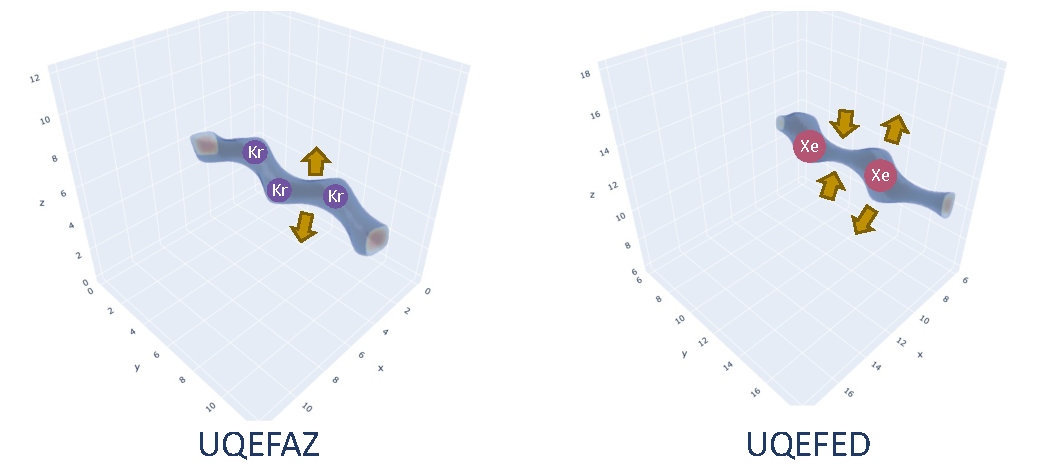
\includegraphics[width=0.95\textwidth]{figures/6-perspectives/KAXQIL_stretch.pdf}
  \caption{ Visualization of the pore size stretching effect using the GrAED algorithm. The xenon increases the LCD value while diminishing the PLD value. }\label{fgr:stretch}
\end{figure}

Now that we identified two completely different diffusion behaviors, we can extrapolate these results to hypothetical conditions. For instance, if there is a relation between the quantity of xenon inside the pores and the structural similarity toward UQEFED, then the material could kinetically limit the adsorption of xenon at a high loading of xenon. In other words, it could be kinetically harder to adsorb xenon at higher xenon loadings. But at lower xenon loading, it also means that there is no diffusion limitations as is suggested by the very steep mass transfer zone on the breakthrough curve of xenon on the Figure~\ref{fgr:sbmof_breakthrough}. If we connect this result on the influence of flexibility on the transport properties to the one obtained on the adsorption process itself, the adsorption of xenon is also much more thermodynamically favorable at higher values of xenon loading. There seems to be a complex thermodynamics-kinetics trade-off as we articulated in the previous chapter since KAXQIL and UQEFED are structurally quite similar, but it occurs at higher partial pressure in xenon. At an industrial point of view, the inclusion of transport effects in the analysis highlights additional cost in adsorbing xenon at high loading values if this theoretical study is confirmed by experiments.

By using simple simulation methods (Widom insertion and MD) on rigid structures, I probed the effects of flexibility on both the adsorption and transport properties using experimentally resolved structures in different adsorption conditions. This study sheds light on the mystery around the experiment-theory discrepancies and opens up opportunities to understand similar problematic systems. In this study, I relied on the experimental data that was published on the SBMOF structure, the same resources are not always available for other systems and maybe an effort of data generation using either experiments or simulations should be performed in these cases. If generalized, this approach can even be automatically applied on a series of structures, opening up the possibility of ``flexibility-aware'' screenings in the future. Aware of the importance of both flexibility and transport effects, other studies have tried to incorporate both in a small-scale screening process.\autocite{Stanton_2022} The authors used a flexible forcefield MD simulations to determine the diffusion coefficient and DFT calculations at the adsorption site to assess the adsorption performance. The main issue of this method is its computational cost, but it can be an alternative solution to the one introduced here, when no prior knowledge is available on the structure’s flexibility. 

\section{Noble Gas Polarizability}

The last but not the least effect that could influence greatly the adsorption performances is, the level of theory behind the interaction energy modelization. In most screening studies, we use (me included) very low-level classical theories to describe the guest--host interactions, because of the low computational cost associated to it. To improve the description, some studies focus on a few specific structures and use higher levels of theory such as DFT calculations. However, the prohibitive computational cost of these methods makes it hard to deploy it in high-throughput screenings. 

But first, we should identify the limits of molecular modeling in the current screening methodologies before exploring higher cost methods. This work is actually motivated by the recent advances in experimental design of nanoporous materials for Xe/Kr separation. The most selective materials are based on highly polar groups or exposed open-metal sites.\autocite{Li_2019,Pei_2022} The polarization is, therefore, central in these materials, but it is not well described by a simple Lennard-Jones potential especially when it is induced by high partial charge values (open-metal site or polar groups). 

For this reason, it is necessary to develop a polarizable forcefield that includes the effect of the surrounding partial charges into the guest--host interactions. The difference of polarizability between xenon and krypton could let new materials emerge. The best material ranking obtained by this type of screening would be completely different from the standard one. In this section, I will introduce the problem of current methodologies through an experiment-theory comparison, and then I will introduce possible methodologies that could be used to take into account the polarization in the currently used Lennard-Jones potentials.

\subsection{Problem definition}

\begin{figure}[ht]
  \centering
  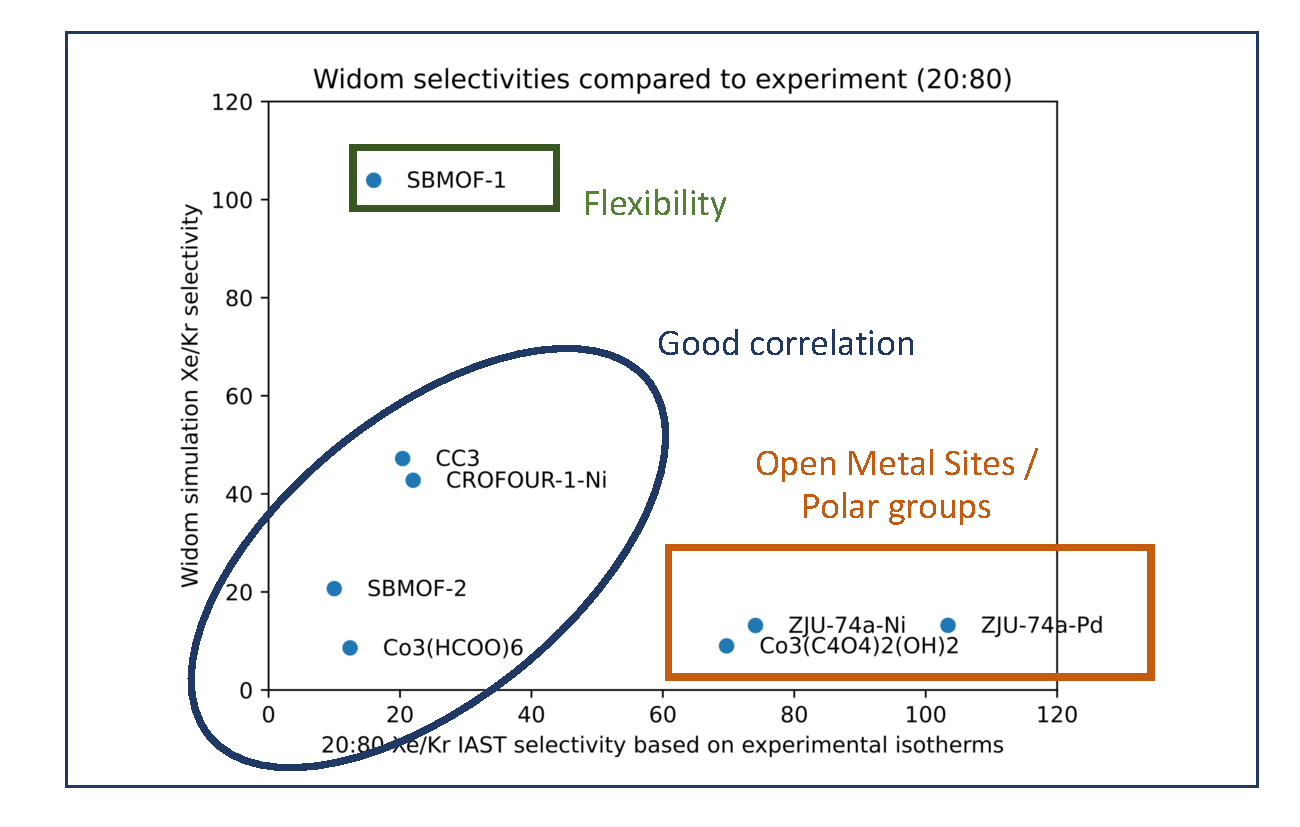
\includegraphics[width=0.7\textwidth]{figures/6-perspectives/exp_theory_discrepancies.pdf}
  \caption{ Comparison between the selectivity values obtained experimentally and computationally. The structures are split in three categories depending on the difference between experiments and theory. We can explain the case of SBMOF-1 by its flexibility. The discrepancies for the materials in the lower right correspond to the ones introduced by Li et al. and Pei et al.,\autocite{Li_2019,Pei_2022} and the difference can be explained by the polarization that is not included in the level of theory considered. \todo{higher resolution+change xaxis (IAST)} }\label{fgr:exp_theory_discrepancy}
\end{figure}

If we consider the selectivity of good materials for xenon/krypton separation that are often presented in the literature, the materials named \ce{Co3(HCOO)6},\autocite{Wang_2014} CC3,\autocite{Chen_2014} SBMOF-2,\autocite{Chen_2015} CROFOUR-1-Ni,\autocite{Mohamed_2016}  SBMOF-1,\autocite{Banerjee_2016} \ce{Co3(C4O4)2(OH)2}\autocite{Li_2019} and ZJU-17a\autocite{Pei_2022} often appear as top separation materials.
When comparing their selectivity values obtained by a Widom insertion with the UFF forcefield to the experimental values as shown on the Figure~\ref{fgr:exp_theory_discrepancy}, there is generally a good correlation, however, in some cases like SBMOF-1, other effects could explain the difference observed (see thr previous section on flexibility). In other cases, it is the polarization effect that was not taken into account and could in fact explain the difference. To better understand this phenomenon, I will describe the two papers that found record-breaking Xe/Kr selectivity values based on polar hydroxyl groups and open metal sites.

The first paper of Li et al.\autocite{Li_2019} published in 2019 introduced a squarate-based MOF with a Xe/Kr selectivity of $69.7$ for a 20:80 binary mixture estimated by the ideal adsorbed solution theory (IAST)\autocite{Cessford_2012}. The authors explained this outstanding xenon affinity by two factors: a pore size close to the kinetic diameter of a xenon and the stabilization effect of the hydroxyl group. DFT calculations determined binding energies of the order of \SI{44.1}{\kJ\per\mole} for xenon and \SI{33.7}{\kJ\per\mole}, which suggests a separation process of enthalpic nature (usually the case for highly selective materials). Because of the high electronegativity of the oxygen atom, the hydroxyl group pointing to the pore center (as illustrated on the Figure~\ref{fgr:jacs_li_str}) interacts strongly with the xenon through a permanent dipole--induced dipole interaction (introduced in the section~\ref{sct:interaction}). This high xenon affinity is illustrated by the experimental isotherms of the Figure~\ref{fgr:jacs_li_isotherm}. On the other hand, the pore wall creates unidimensional channels that present adsorption pores with a \SI{4.1}{\angstrom}$\times$\SI{4.3}{\angstrom} size, which is very close to the xenon kinetic diameter of about \SI{4.0}{\angstrom}. 

\begin{figure}[ht]
  \centering
  \begin{subfigure}[b]{0.34\textwidth}
    \centering
    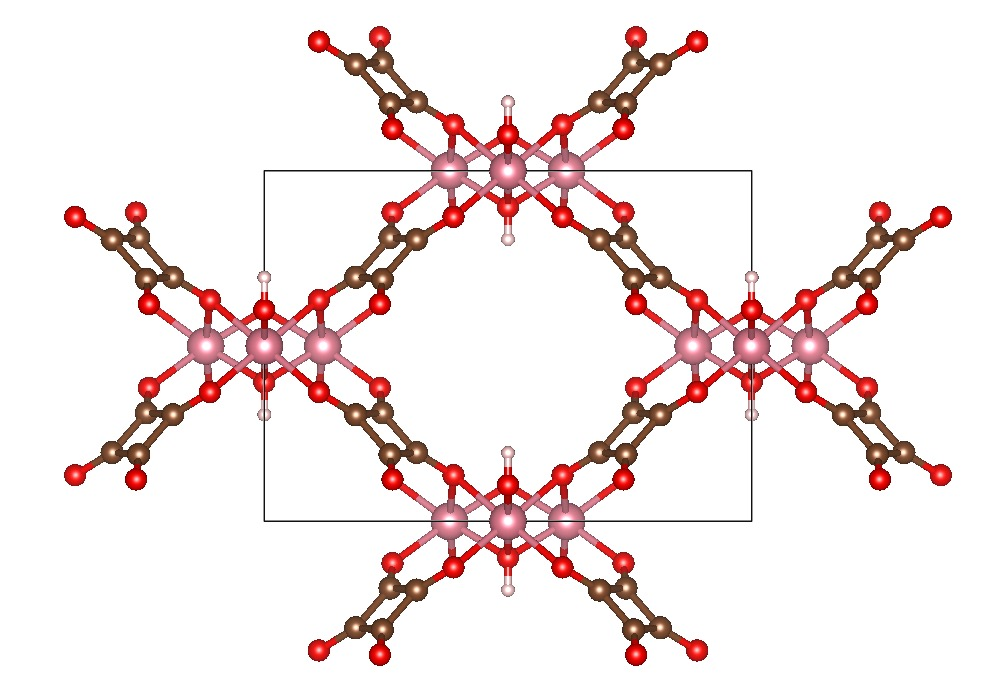
\includegraphics[width=\textwidth]{figures/6-perspectives/jacs_li.jpg}
    \caption{VESTA visualization\autocite{VESTA}}\label{fgr:jacs_li_str}
  \end{subfigure}
  \hfill
  \begin{subfigure}[b]{0.34\textwidth}
    \centering
    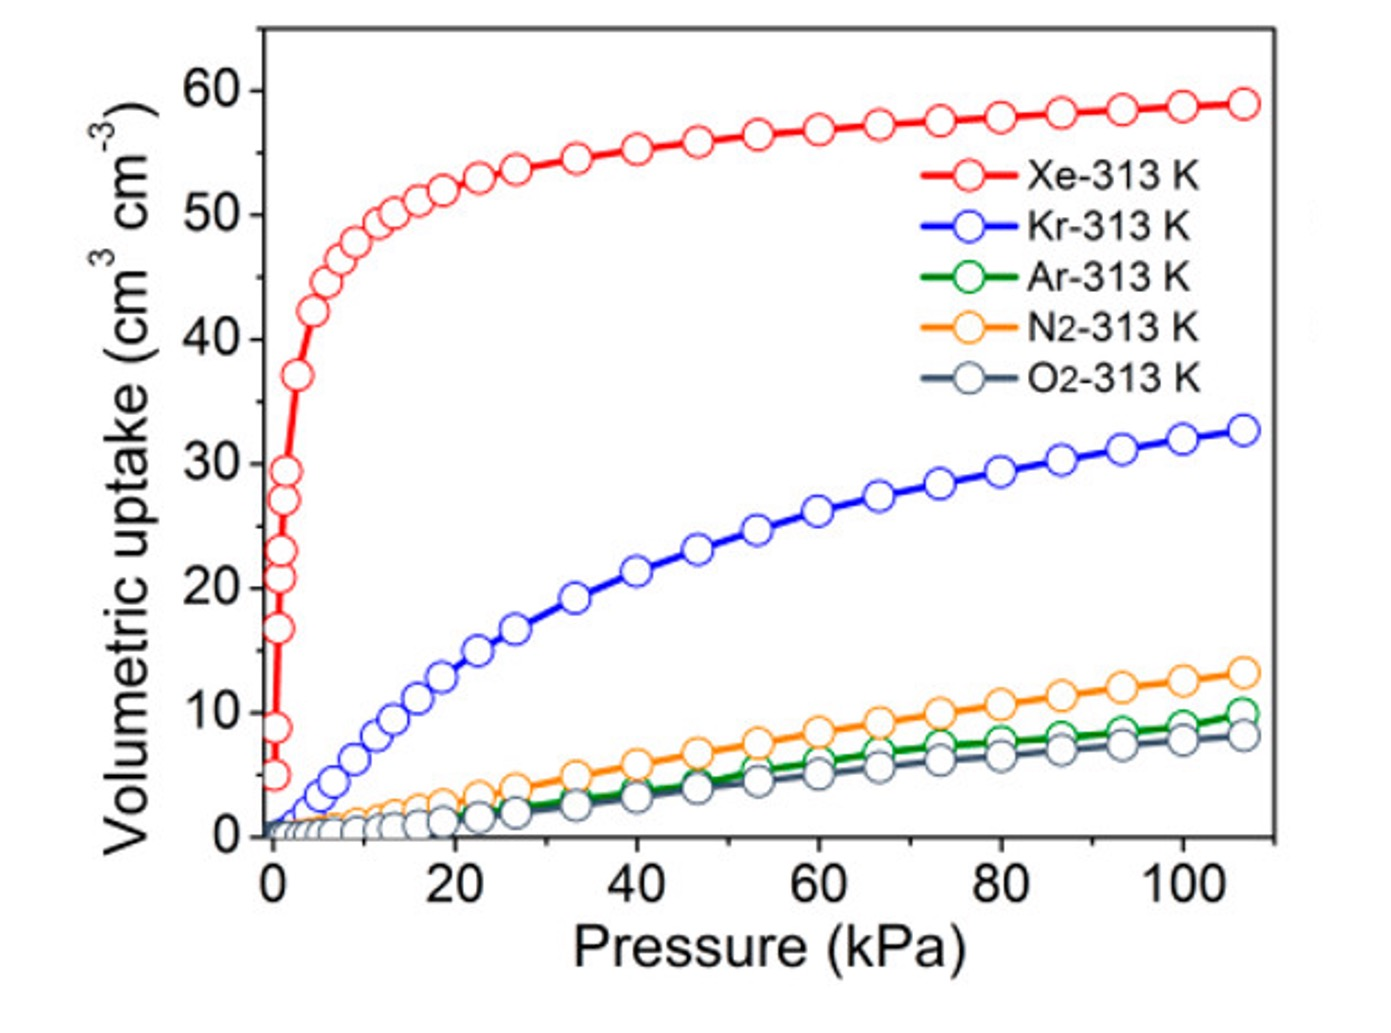
\includegraphics[width=\textwidth]{figures/6-perspectives/jacs_li_isotherm.jpg}
    \caption{Adsorption isotherms}\label{fgr:jacs_li_isotherm}
  \end{subfigure}
  \hfill
  \begin{subfigure}[b]{0.25\textwidth}
    \centering
    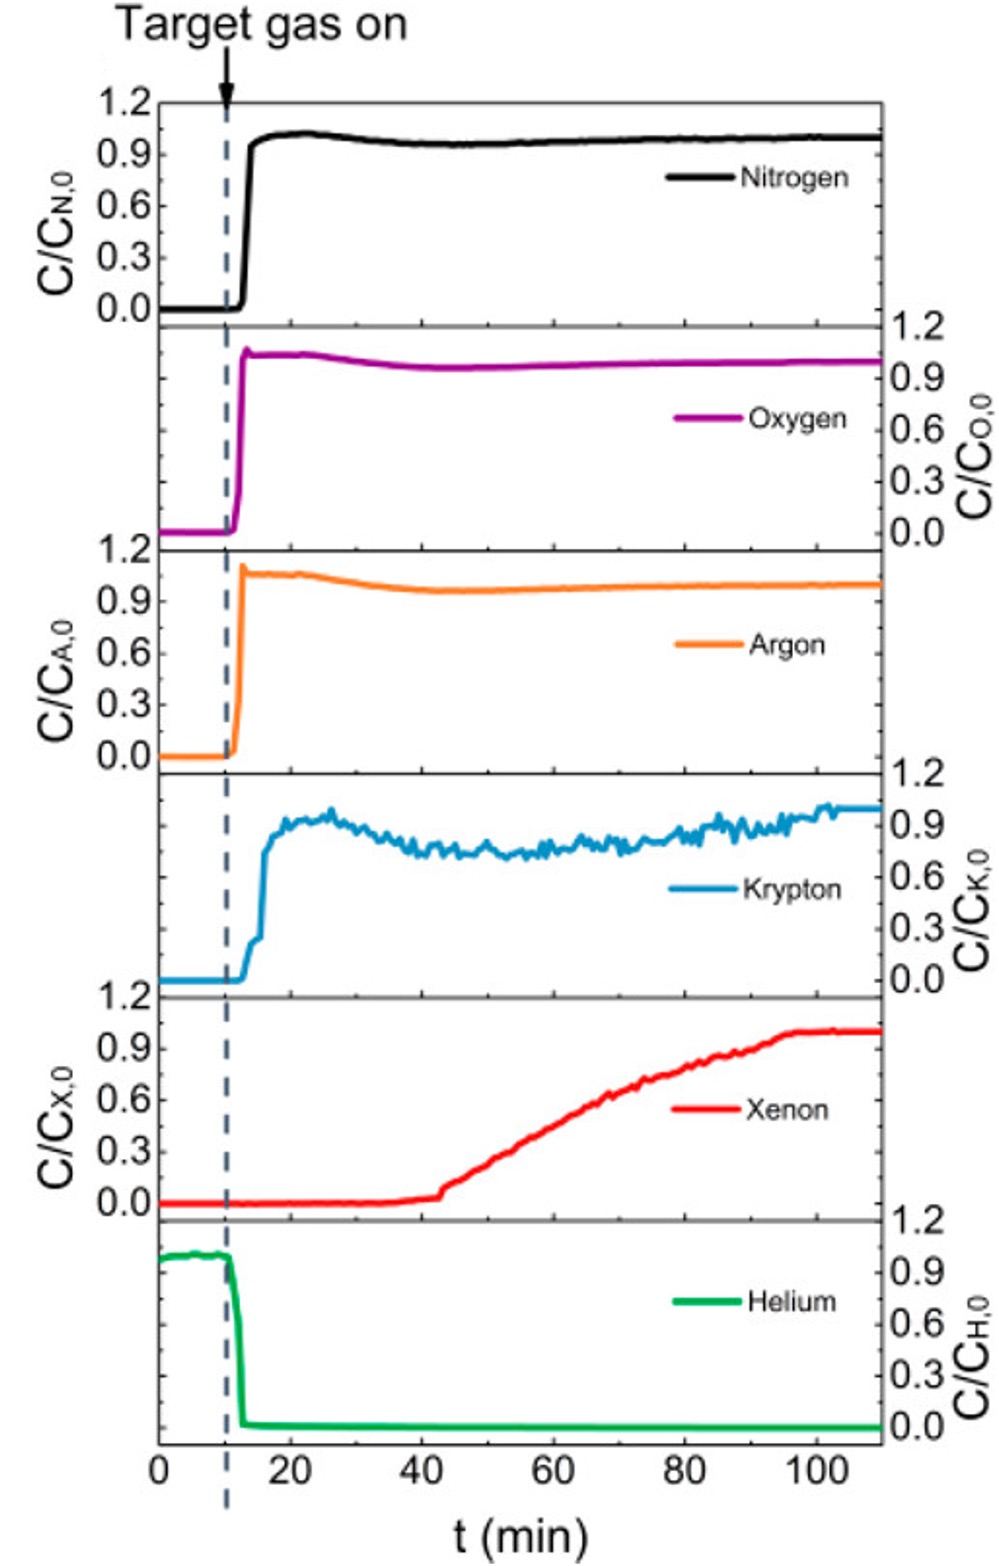
\includegraphics[width=\textwidth]{figures/6-perspectives/jacs_li_breakthrough.jpg}
    \caption{Breakthrough curves}\label{fgr:jacs_li_breakthrough}
  \end{subfigure}
  \caption{ (a) Representation of the squarate-MOF \ce{Ce3(C4O4)2(OH)2} structure with the color code: brown for C, white for H, red for O, pink for Co. We can see the hydroxyl group to which the authors attribute the high Xe/Kr selectivity. (b) Mono-component adsorption isotherm measured experimentally for Xe, Kr, Ar, \ce{N2} and \ce{O2}. (c) Experimental breakthrough curves for a gas mixture with 400 ppm Xe and 40 ppm Kr balanced with dry air. Reprinted with permission from Ref.~\cite{Li_2019} copyright \copyright\ 2019 American Chemical Society. }\label{fgr:jacs_li}
\end{figure}

Finally, if we look at the breakthrough experiment data (on the Figure~\ref{fgr:jacs_li_breakthrough}), we observe a rather slow release of xenon in the mass transfer zone, which suggests a rather low xenon diffusion coefficient in this material.It seems that the diffusion limitation occurs even at very low xenon partial pressure (400 ppm) in this material. This was not the case for SBMOF-1, as the xenon breakthrough curve was much steeper (rapid mass transfer) as shown on the Figure~\ref{fgr:sbmof_breakthrough}. To have a closer look at the transport effect in this squarate-MOF, we should carry out similar simulations as for SBMOF-1 with a polarizable forcefield. 

In the second work,\autocite{Pei_2022} Pei et al. introduced two Hofmann-type MOFs with record-breaking Xe/Kr selectivity values. The first Co/Ni-based MOF, called ZJU-74a-Ni, has an estimated IAST selectivity of $74.1$ for a Xe/Kr binary mixture of composition 20:80 at \SI{1}{\bar} and \SI{298}{\kelvin}, while the second Co/Pd-biased MOF, ZJU-74a-Pd, displays a selectivity of $103.4$ in the same ambient-pressure conditions. As shown on the Figure~\ref{fgr:jacs_pei_iast}, the IAST selectivity of ZJU-74a-Pd is not always that high and can decrease to $30$ at very low-pressure conditions. The authors attribute the record-breaking selectivity values of these materials by a size close to the kinetic diameter of Xe and above all the increased interaction with the open metal site either be it the nickel or the palladium atoms. The Horvath–Kawazoe method gave a pore size of \SI{4.0}{\angstrom} and \SI{3.8}{\angstrom} for respectively the Ni and Pd-based MOFs. And the xenon binding energy was evaluated to be around \SI{38}{\kJ\per\mole} for ZJU-74a-Ni using a UFF-based method. We can note that this value is much lower than the one obtained for the squarate-based MOF. Since the experimental performance is much higher, this is probably due to the level of theory they employed probably to save time. This material needs to be tested with either a DFT method in order to find the real binding energy. 

\begin{figure}[ht]
  \centering
  \begin{subfigure}[b]{0.34\textwidth}
    \centering
    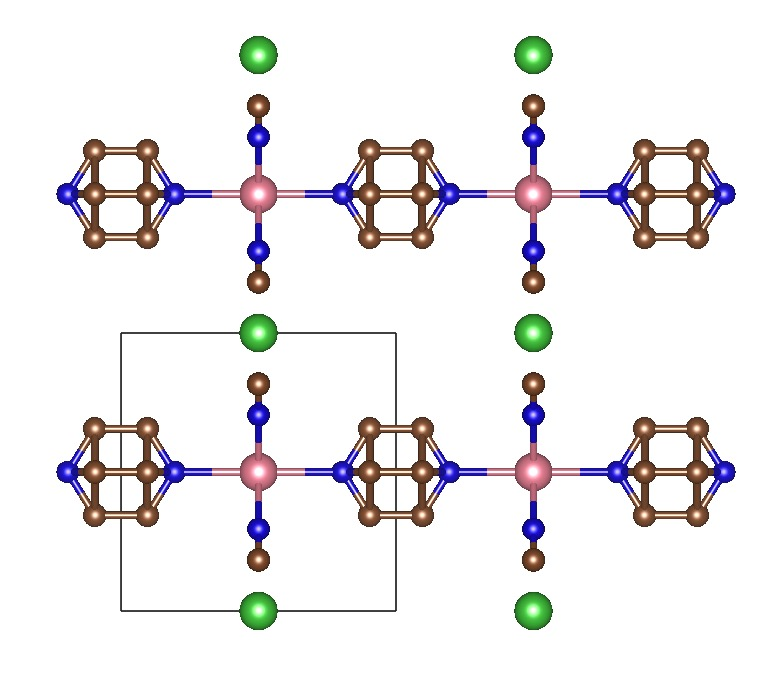
\includegraphics[width=\textwidth]{figures/6-perspectives/jacs_pei.jpg}
    \caption{VESTA visualization\autocite{VESTA}}\label{fgr:jacs_pei_struc}
  \end{subfigure}
  \hfill
  \begin{subfigure}[b]{0.34\textwidth}
    \centering
    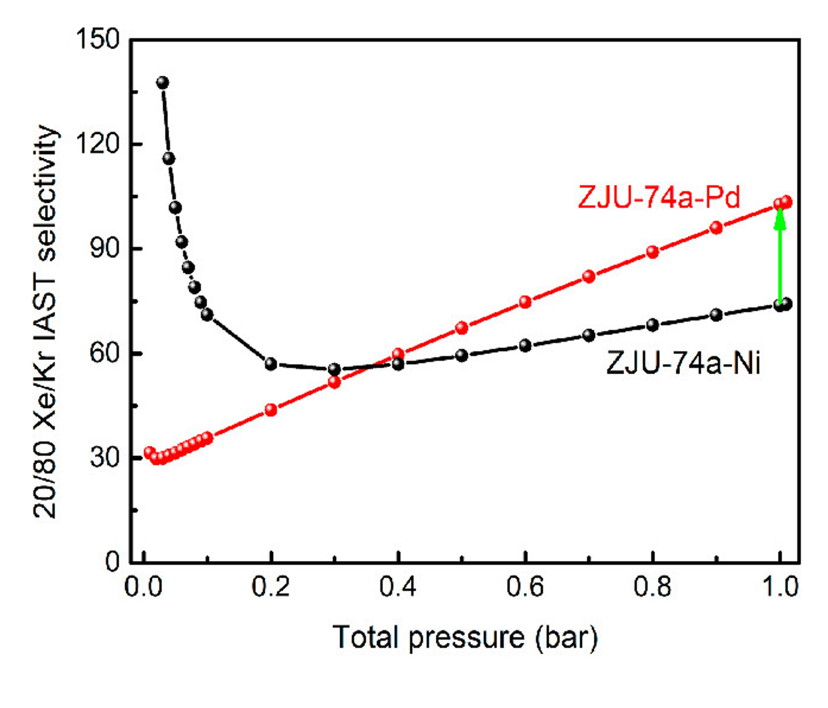
\includegraphics[width=\textwidth]{figures/6-perspectives/jacs_pei_iast.jpg}
    \caption{IAST selectivity}\label{fgr:jacs_pei_iast}
  \end{subfigure}
  \hfill
  \begin{subfigure}[b]{0.25\textwidth}
    \centering
    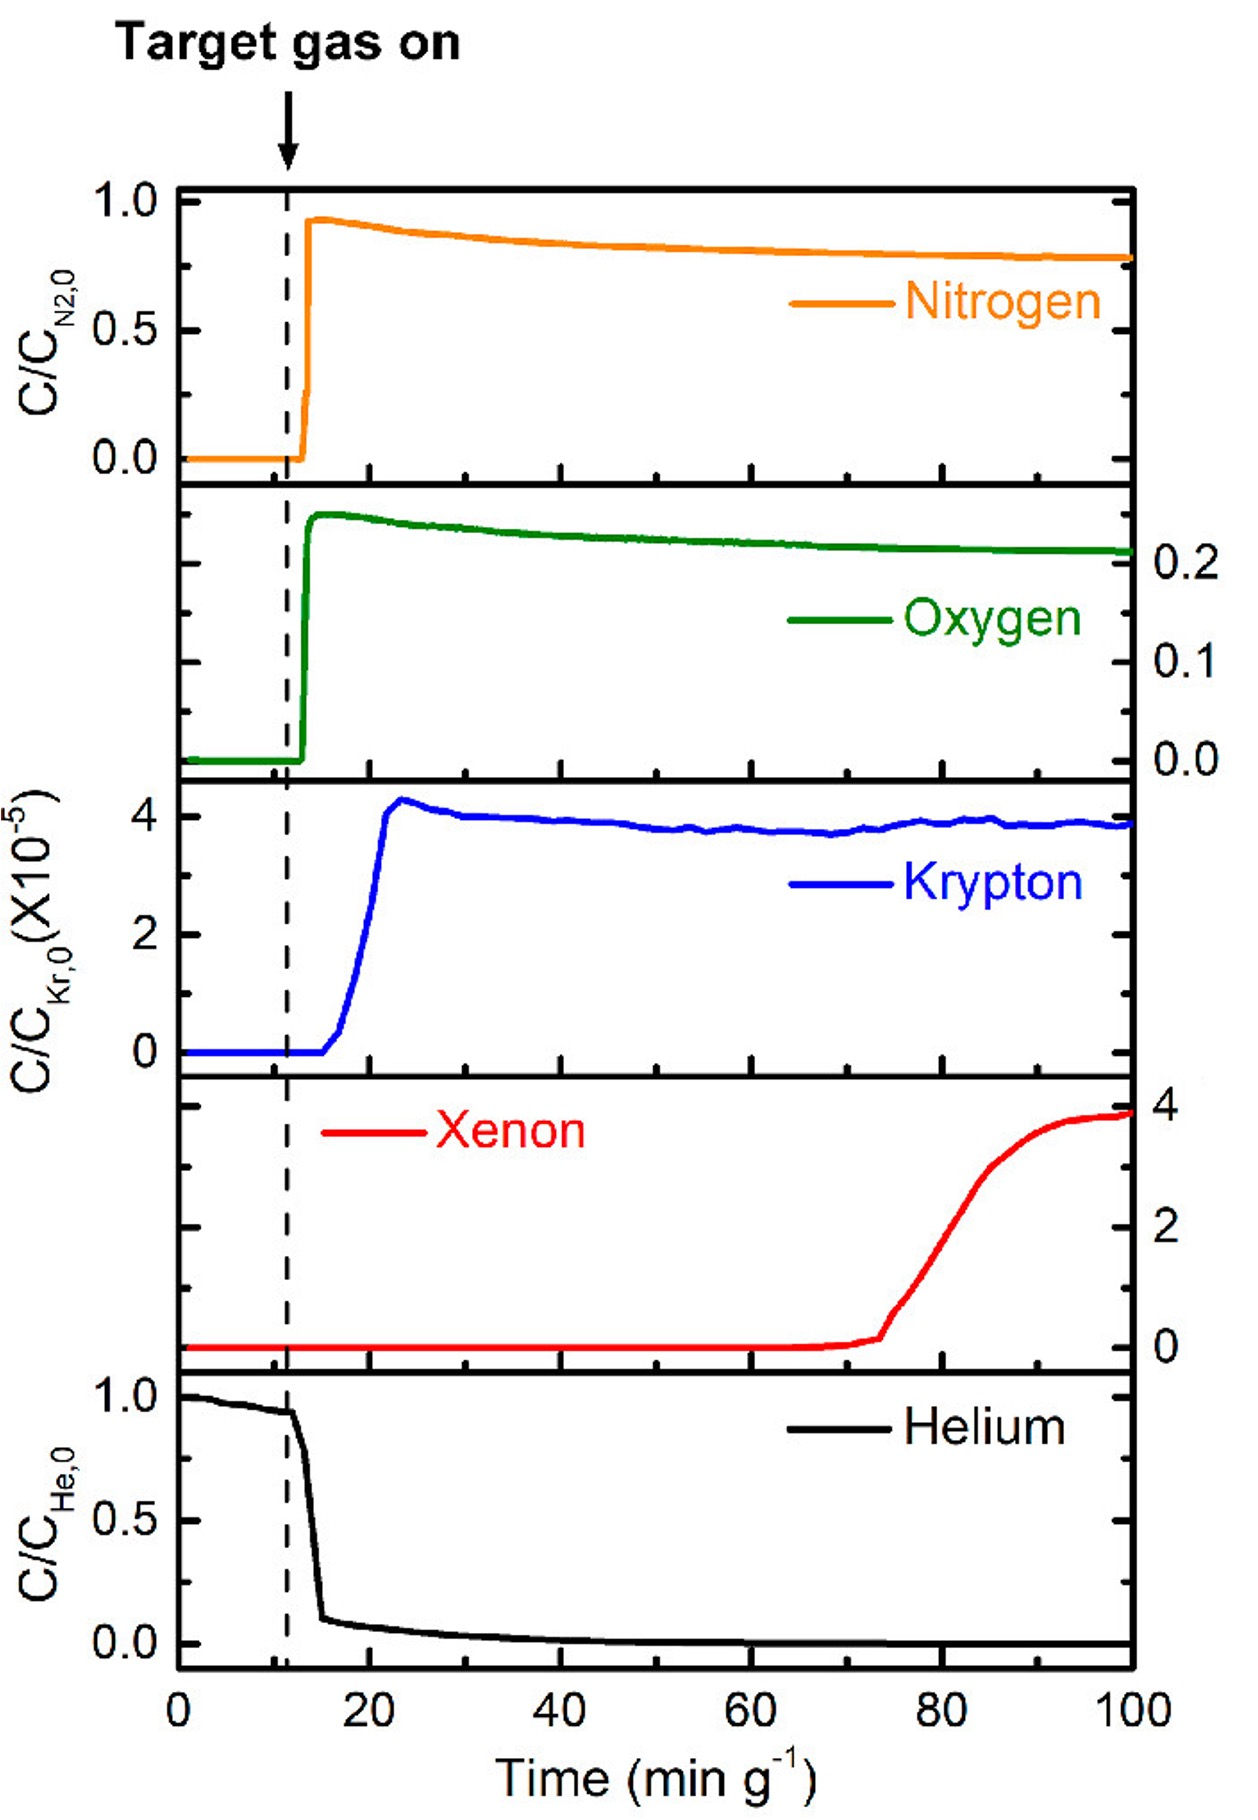
\includegraphics[width=\textwidth]{figures/6-perspectives/jacs_pei_breakthrough.jpg}
    \caption{Breakthrough curves}\label{fgr:jacs_pei_breakthrough}
  \end{subfigure}
  \caption{ (a) Representation of the ZJU-74a-Ni structure with the color code: brown for C, white for H, red for O, pink for Co, green for Ni. We can see the open metal sites or coordinatively unsaturated nickel metals that could interact with an adsorbate in the center of the pore. (b) Selectivity values at different pressure conditions for a 20:80 Xe/Kr binary mixture calculated by the IAST theory. (c) Experimental breakthrough curves of a gas mixture with 400 ppm Xe and 40 ppm Kr balanced with dry air in ZJU-74a-Pd. Reprinted with permission from Ref.~\cite{Pei_2022} copyright \copyright\ 2022 American Chemical Society.}\label{fgr:jacs_pei}
\end{figure}

Finally, the breakthrough experiment suggests a rather slow mass transfer in the material. However, if compared to the squarate-based material in similar conditions, the mass transfer seems to be much faster, since the mass transfer zone is shorter. ZJU-74a-Pd is, therefore, probably a better material than \ce{Co3(C4O4)2(OH)2} because its better adsorption and transport properties for a Xe/Kr separation. When compared to SBMOF-1 with a rather low xenon partial pressure, there seems to be a slight diffusion limitation phenomenon. The retention of xenon is, on the other hand, longer in ZJU-74a-Pd (around \SI{70}{\s}) than in SBMOF-1 (around \SI{65}{\s}). We probably need more information on the ambient-pressure selectivity of SBMOF-1, to complete the comparison.
This material is also interesting for its robustness in different pH, humidity and radiation conditions, which makes it a material of choice in nuclear installations to capture the xenon produced by the nuclear reactions.

These two studies show clearly the failure of current screening methodologies to find materials whose performance is due to polarization effects. In the next and final discussion, we will introduce some methods of incorporating polarization into Lennard-Jones potentials that could be used in a screening procedure.

\subsection{Studying the polarization}

The physical reason behind considering the polarization effect for xenon/krypton separation is to exploit the difference of polarizability between Xe (\SI{4.0}{\cubic\angstrom}) and Kr (\SI{2.5}{\cubic\angstrom})\autocite{Olney1997} at its full potential. And in a broader perspective, the order of magnitude of the induction energy is actually higher than other standard van der Waals energies as explained in the section~\ref{sct:interaction}. For instance, the ion--induced dipole interaction is said to be of the order of 40-600~\si{\kJ\per\mol}. In the case of ZJU-74a-Ni, the Ni\ex{2+}---Xe---Ni\ex{2+} interaction at the origin of selectivity is precisely this type of interaction, which mostly explains the experimental values of selectivity. The incorporation of polarization in the screening procedure could completely change the type of structures obtained and the type of the interactions at play.

With this in mind, Becker et al. carried out an interesting study on a series of MOF materials with a high density of open-metal sites, the M-MOF-74 with M = Co, Cr, Cu, Fe, Mg, Mn, Ni, Ti, V, and Zn.\autocite{Becker_2017} The authors found that by adding a potential induced by the surrounding partial charges to a modified LJ potential, they could reproduce the \ce{CO2} and \ce{CH4} experimental isotherm data for this series of MOFs. They also showed that the standard UFF forcefield does no describe the adsorption behavior of \ce{CO2} on the open-metal sites, hence missing out on a strong adsorption site at infinite dilution. 

This new method is based on the procedure developed by Lachet et al.\autocite{Lachet_1998}. This procedure is based on the induced dipole method where the induction energy $U\e{ind}$ is expressed as follows:

\begin{equation}
  U\e{ind} = -\frac{1}{2} \sum_{i=1}^{N} \boldsymbol{\mu}_i \cdot \mathbf{E}_i^0
\end{equation}
where $\boldsymbol{\mu}_i$ is the induced dipole, and $\mathbf{E}_i^0$ is the electric field created by the surrounding atoms' partial charges on the particle $i$. Since the induced dipole also interacts with the surrounding induced dipoles $j\neq i$, the induced dipole is usually calculated using a back-propagation algorithm as described in the Ref.~\cite{Lachet_1998}. However, back-propagation was found to only account for less than {5\%} of the total induction energy. For this reason the equation can be simplified to the simple interaction between the induced dipole and the surrounding electric field without taking into account the induced-dipole--induced-dipole interactions. Moreover, by skipping the bacpropagation step, we can save valuable computation time in a screening. The induction energy can then be simply expressed as follows:

\begin{equation}
  U\e{ind} = -\frac{1}{2} \sum_{i=1}^{N} \alpha_i {\left\lvert\mathbf{E}_i^0\right\rvert}^2
\end{equation}

Since a part of the induction energy is already contained in the Lennard-Jones potential, the authors rescaled the LJ parameters to remove the induction part from the LJ energy. This part seems to be system-dependent and could in fact be questionable since we can use it to fit to experimental data without solid theoretical reasons to back it. To do it preperly, one should design a forcefield around this concept in order to tweak the LJ-parameters according to a given experimental data as it is usually done in any forcefield development. 

If we manage to adapt this method to the xenon/krypton separation case, it could be possible to carry out screenings that find materials comparable to ZJU-74a-Pd. To further optimize the screening approach, we could also find materials with a certain pore size and that contain open metal sites within a database, and then evaluate this restricted list using higher-level methods. 

\todo{Estimate the induction energy for ZJU and squarate}


\OnlyInSubfile{\printglobalbibliography}

\end{document}
